\subsection{UTS}
In this section, we demonstrate the UTS-GLB performance by showing
three figures, one per each architecture. On each architecture, we
compare the legacy code to the GLB implementation. One thing to note is that the legacy code is a highly tuned parallel implementation of UTS and it won the HPCC2012 performance award~\cite{tardieu-petascale}.
On each figure, the x-axis represents the number of places; the primary y-axis (the left y-axis) represents the number of UTS nodes counted per second; the secondary y-axis (the right y-axis) represents the efficiency, which is calculated by how many nodes counted per second per place. A straight line whose slope is 1 along the primary y-axis indicates a linear speedup and a horizontal line on the secondary y-axis indicates the implementation scales perfectly. In the following discussion, we refer to UTS legacy code by UTS and refer to UTS GLB code by UTS-G.

\begin{figure}
\centering
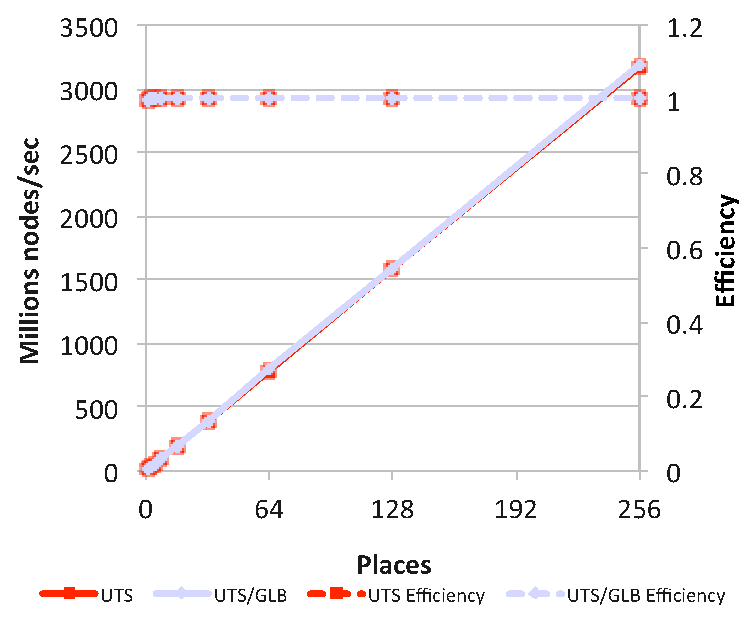
\includegraphics[width=2.25in]{./ppaa2014_figures/uts_p7ih.eps}
\caption{UTS/UTS-G Performance Comparison (on Power~775)}
\label{fig:perf:uts-p7ih}
\end{figure}

Figure ~\ref{fig:perf:uts-p7ih} shows the performance comparison for UTS and UTS-G on Power~775 up to 256 cores. UTS and UTS-G both achieve linear speedup and their efficiencies stay at 1, which means they both achieve perfect scaling.  

\begin{figure}
\centering
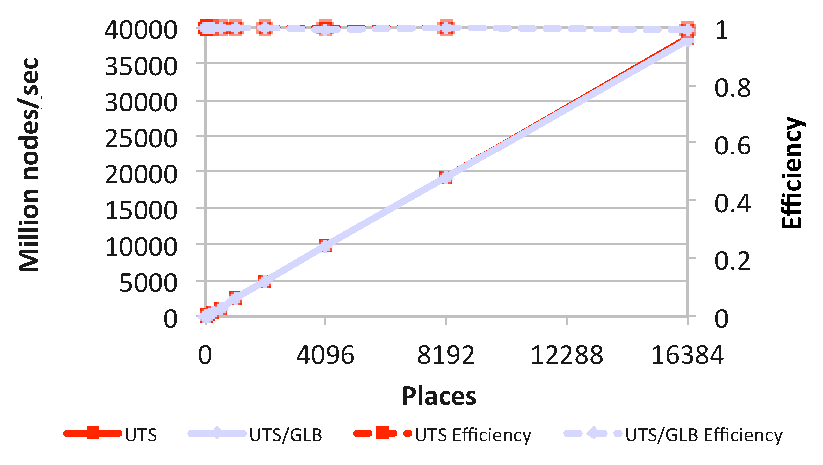
\includegraphics[width=2.55in]{./ppaa2014_figures/uts_bgq.eps}
\caption{UTS/UTS-G Performance Comparison (on Blue~Gene/Q)}
\label{fig:perf:uts-bgq}
\end{figure}
Figure ~\ref{fig:perf:uts-bgq} shows the performance comparison for UTS and UTS-G on Blue~Gene/Q up to 16384 cores. UTS and UTS-G both achieve linear speedup and perfect scaling. 

\begin{figure}
\centering
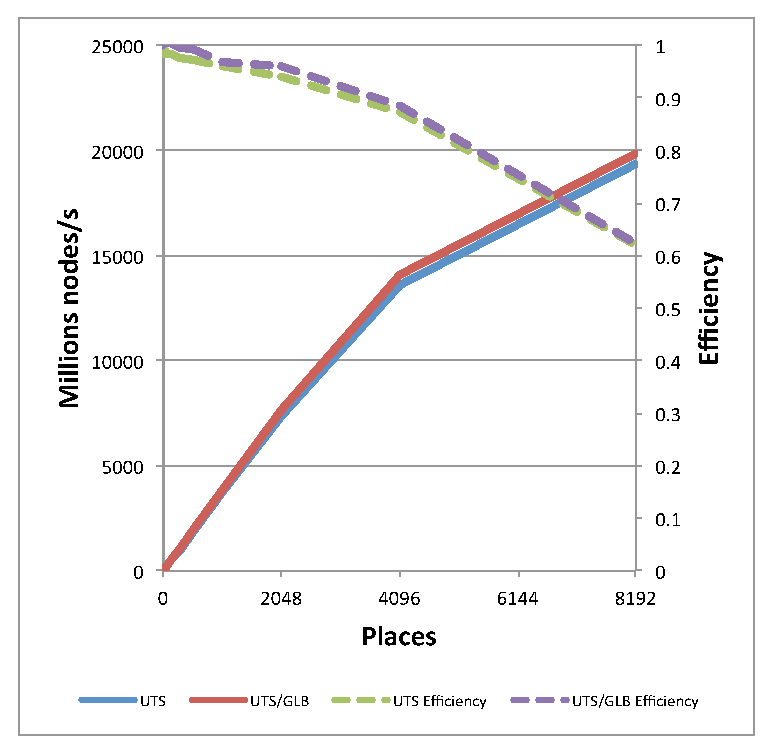
\includegraphics[scale=0.35]{./ppaa2014_figures/uts_k.eps}
\caption{UTS/UTS-G Performance Comparison  (on K)}
\label{fig:perf:uts-k}
\end{figure}
Figure ~\ref{fig:perf:uts-k} shows the performance comparison for UTS and UTS-G on Blue~Gene/Q up to 8192 cores. UTS and UTS-G perform well up to 4096 cores (i.e., almost linear speedup and efficiency stays above 0.9). When running on more than 4096 cores, both UTS and UTS-G drop their efficienies to 0.6. We are still investigating why there is a sudden performance drop on K.

\textbf{Summary} UTS-G achieves near linear speedup and perfect scaling on both Power~775 (up to 256 cores) and Blue~Gene/Q (up to 16384 cores). On all three architectures, UTS-G achieves similar (or better) performance compared to UTS, a highly tuned award-winning implementation.


\subsection{BC}
In this section, we compare the BC-GLB performance to the BC legacy
code. Two things to note are: (1) the legacy BC code uses a very
different synchronization scheme from the legacy UTS code. In
comparison, the GLB implementation of UTS and BC share exactly the
same synchronization scheme (i.e., the underlying GLB library). This
demonstrates GLB is applicable to widely different types of
problems. (2) The legacy BC implementation randomizes which vertices
to compute on each place, which effectively reduces the imbalance
among places. As the number of places increases, such imbalance
decreases. When running on more than 1024 places, BC's performance is
only roughly 15\% worse than then optimal performance (i.e., the longest execution time per place is only 15\% more than the average finishing time across all places). Therefore, it is difficult to improve the performance because the room to improve is limited. 

We demonstrate the UTS-GLB performance by showing six figures, two per each architecture. On each architecture, we first compare performance, then we compare the workload distribution among places.   
On each performance comparison figure, the x-axis represents the number of places; the primary y-axis (i.e., the left y-axis) represents the number of edges traversed per second; the secondary y-axis (i.e., the right y-axis) represents its efficiency, which is calculated by number of edges traversed per second per place. A straight line whose slope is 1 along the primary y-axis indicates a linear speedup and a horizontal line along the secondary y-axis indicates the implementation scales perfectly. To understand how effective GLB is at balancing the workload compared to the legacy code, we also plot the workload distribution graphs. On each workload distribution graph, we bar-plot the calculation time on each place and bundle them together. The more even workload distribution graph appears, the more balanced workload is. A rectangular visualization indicates the perfect load-balancing. We also show the mean and standard deviation of the workload distribution on each figure. In the following discussion, we refer to BC legacy code as BC and refer to BC-GLB code as BC-G. 

\begin{figure}
\centering
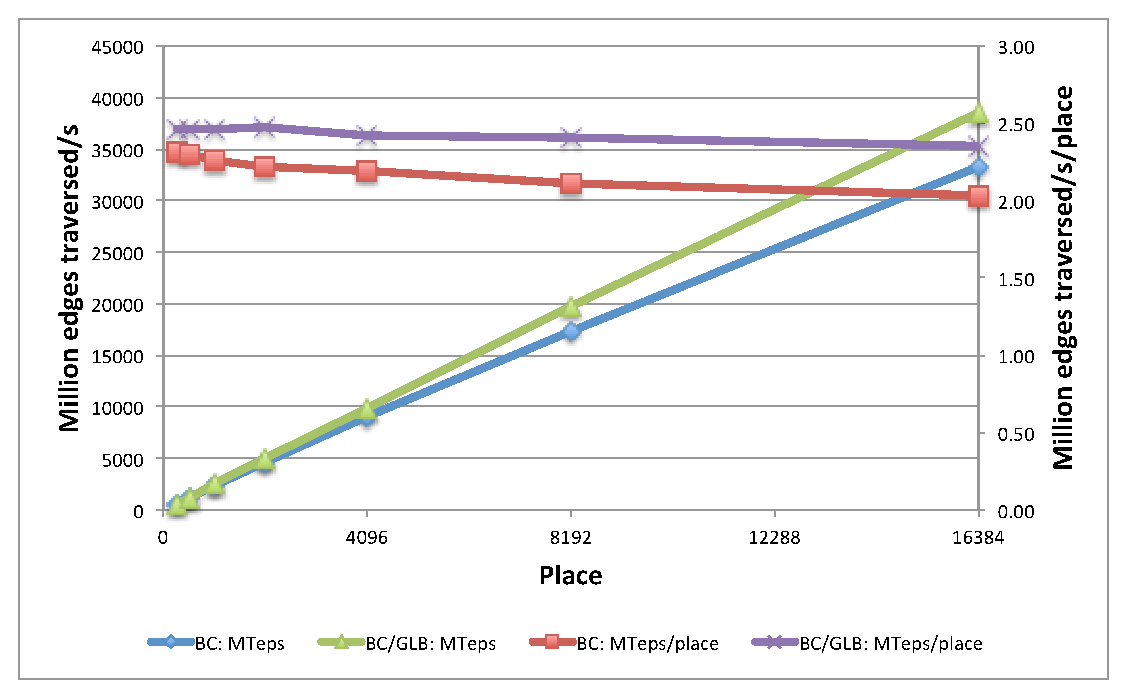
\includegraphics[width=2.25in]{./ppaa2014_figures/bc_bgq.eps}
\caption{BC/BC-G Performance (on Blue~Gene/Q)}
\label{fig:perf:bc-bgq}
\end{figure}
Figure~\ref{fig:perf:bc-bgq} shows the BC performance comparison on Blue~Gene/Q. We can see that GLB implementation achieves near linear speedup and near perfect scaling. 



\begin{figure}
\centering
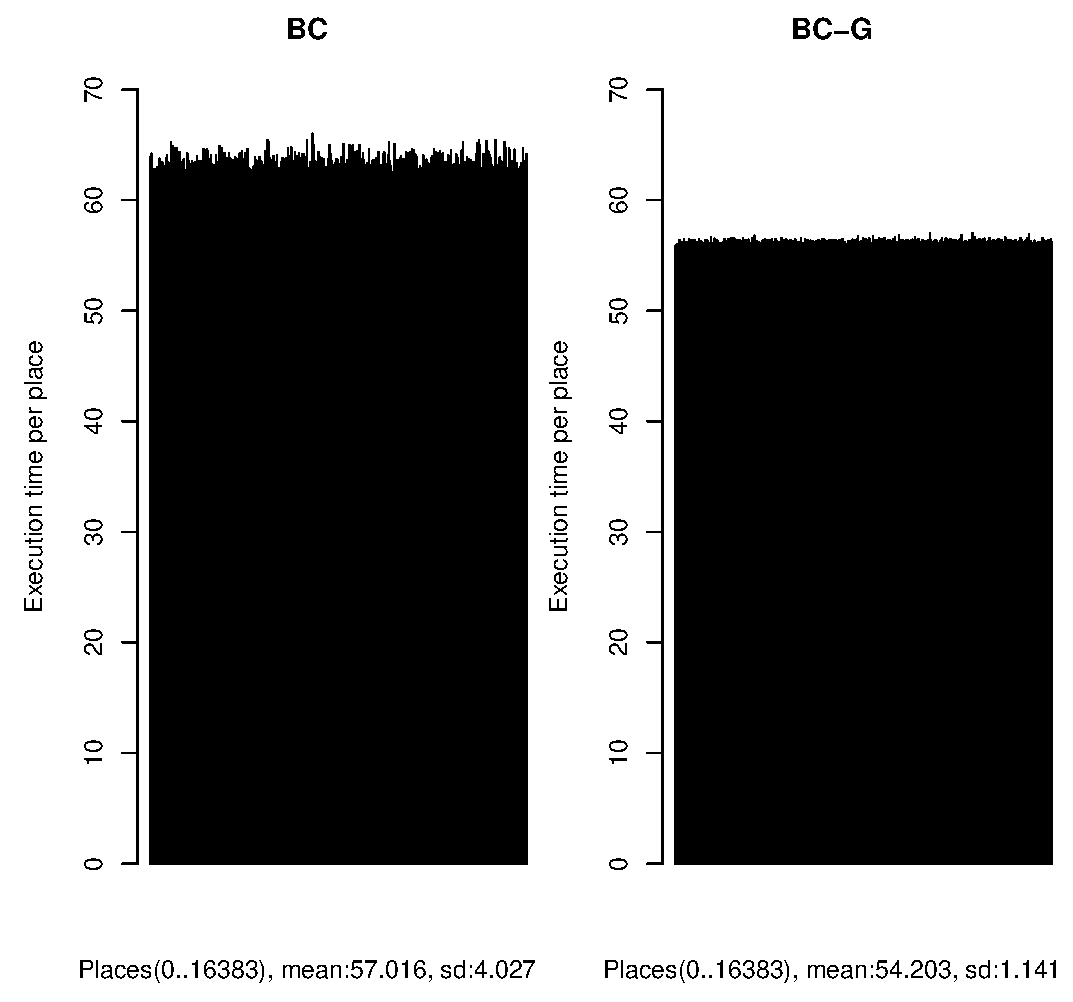
\includegraphics[width=2.25in]{./ppaa2014_figures/bgq_workload.eps}
\caption{BC/BC-G Workload Distribution (on Blue~Gene/Q)}
\label{fig:dist:bc-bgq}
\end{figure}
Figure~\ref{fig:dist:bc-bgq} shows the workload distribution of BC on Blue~Gene/Q. As we can see, BC-G workload distribution is much more even than that of BC, GLB reduces the standard deviation from 4.027 to 1.141. In fact, BC-G finishes calculation in 57.0586 seconds, which is almost equal to the mean of BC computing time accross all places (57.015s). This indicates that BC-G achieves the near perfect load-balancing on Blue~Gene/Q. 


\begin{figure}
\centering
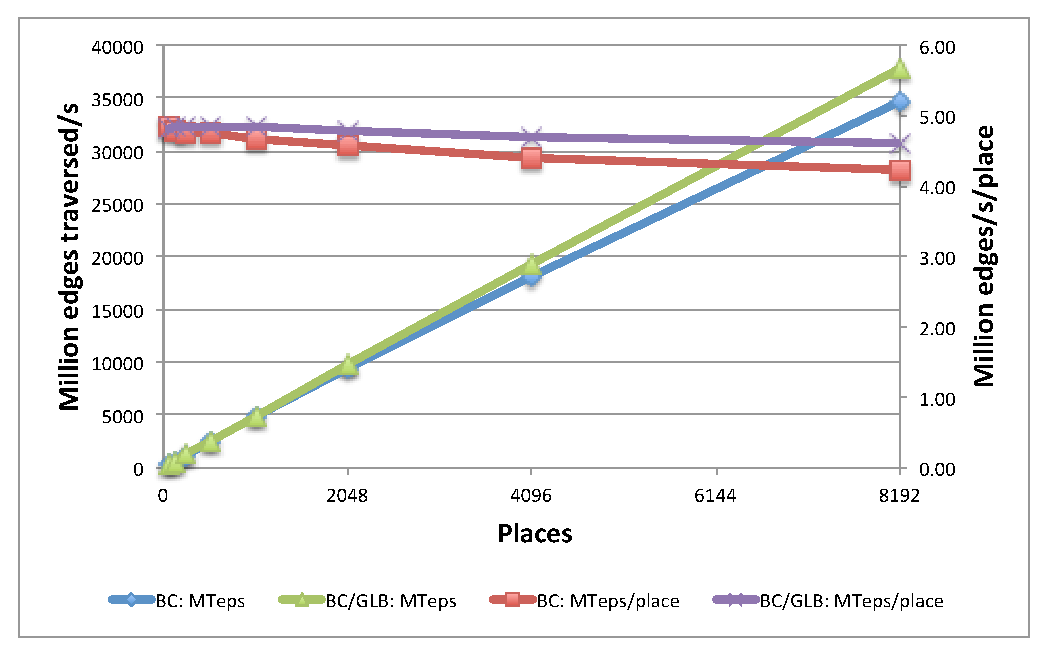
\includegraphics[width=2.25in]{./ppaa2014_figures/bc_k.eps}
\caption{BC/BC-G Performance (on K)}
\label{fig:perf:bc-k}
\end{figure}
Figure~\ref{fig:perf:bc-k} shows the BC performance comparison on K. BC-G also achieves near linear speedup and near perfect scaling (efficiency$>$0.95 up to 8192 places).


\begin{figure}
\centering
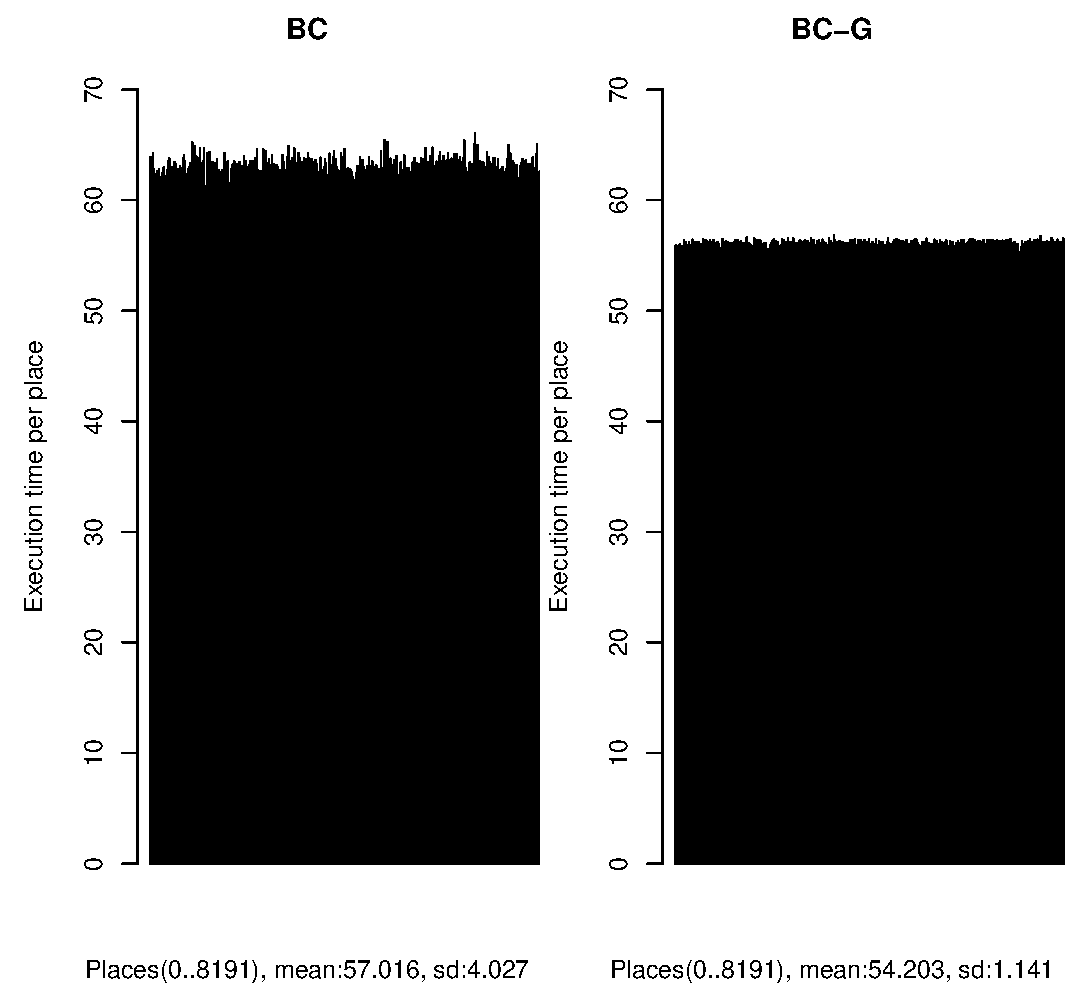
\includegraphics[width=2.25in]{./ppaa2014_figures/k_workload.eps}
\caption{BC/BC-G Workload Distribution (on K)}
\label{fig:dist:bc-k}
\end{figure}
Figure~\ref{fig:dist:bc-k} shows the workload distribution of BC on Blue~Gene/Q. As we can see, BC-G workload distribution is much more even than that of BC on K. BC-G finishes calculation in 58.198729 seconds on 8192 places, which is within 1.5\% of the mean of BC computing time across all places (57.016s). This indicates that BC-G also achieves the near perfect load-balancing on K. 


\begin{figure}
\centering
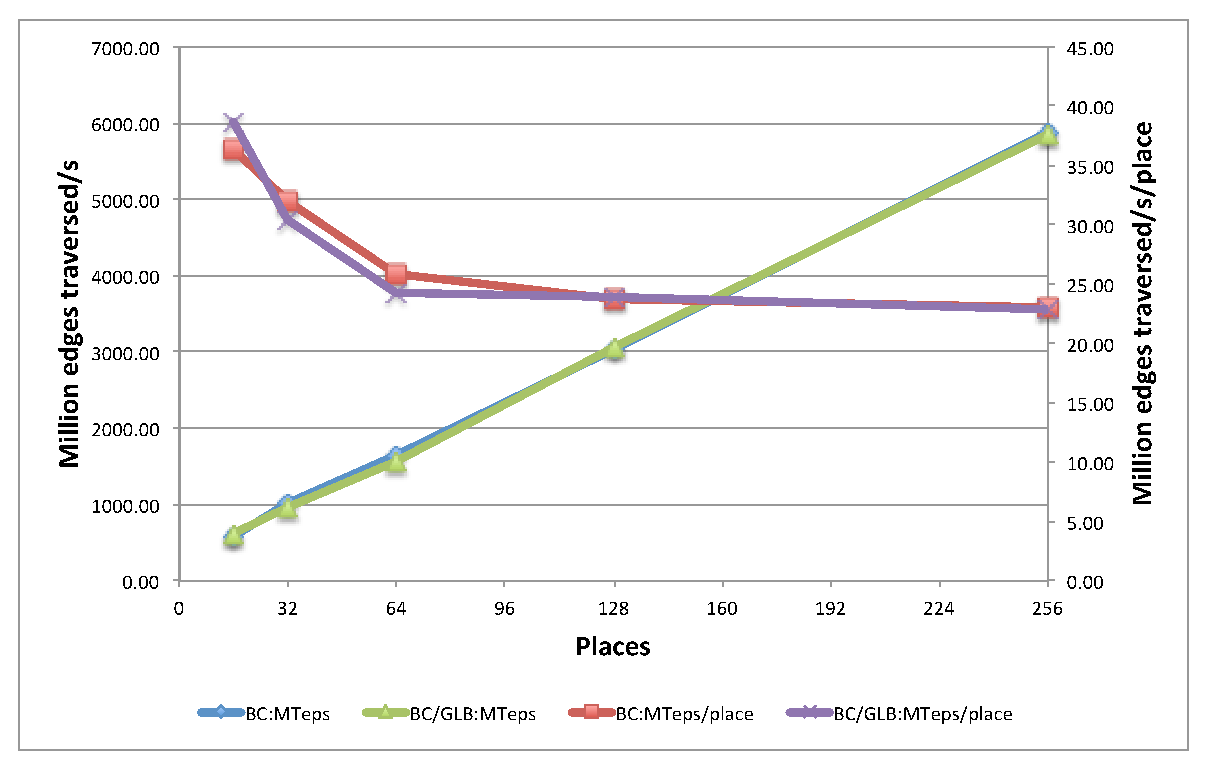
\includegraphics[width=2.25in]{./ppaa2014_figures/bc_p7ih.eps}
\caption{BC/BC-G Performance (on Power 775)}
\label{fig:perf:bc-p7ih}
\end{figure}
Figure~\ref{fig:perf:bc-p7ih} shows the BC performance comparison on
K. Surprisingly, BC-G on Power 775 does not achieve the linear speedup
and perfect scaling as it does on Blue~Gene/Q and on K. That is
because as the number of places increase, the total amount of time to
finish calculating all the vertices also increase even when the graph
stays the same.  Additionally, for the same workload, BC-G spends more
time calculating (on average 5-20\% more) than BC when both run on a
single place. We suspect both problems are due to the overly sensitive
C++ compiler optimizations on Power 755; we are still investigating to
verify this hunch. However, as demonstrated in Figure~\ref{fig:dist:bc-p7ih}, BC-G is very effective at removing the imbalance among workloads, it decreases the workload standard deviation from 58.463 to 1.482.
\begin{figure}
\centering
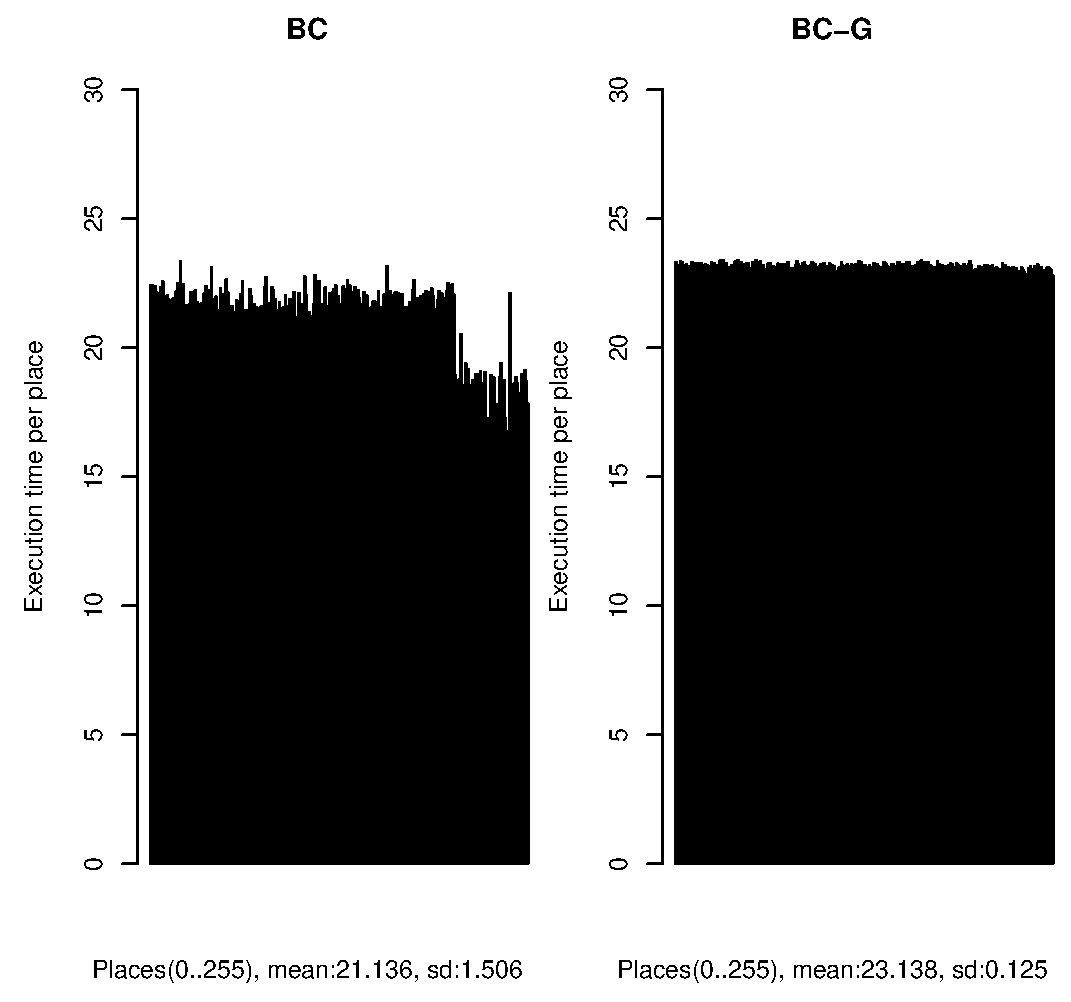
\includegraphics[width=2.25in]{./ppaa2014_figures/p7ih_workload.eps}
\caption{BC/BC-G Workload Distribution (on Power 775)}
\label{fig:dist:bc-p7ih}
\end{figure}

\textbf{Summary}  BC-G constantly outperforms the BC implementation. On Blue~Gene/Q (up to 16384 cores) and K (up to 8192 cores), BC-G achieves the near-optimal speedup, scalability and load-balancing.
